\documentclass{article}
\usepackage{graphicx} % Required for inserting images
\usepackage[english, russian]{babel}

\title{КТ 2 MovieMatch}
\author{Климчук Антонина}

\begin{document}

\maketitle

\section{Цель}
Цель: создать telegram-бота, который поможет компании людей выбрать фильм на вечер так, чтобы всех устроил

\section{Целевая аудитория}
\begin{enumerate}
    \item Любая компания, которая не всегда может найти фильм для просмотра всем вместе
    \item Человек, у которого закончились идеи о том, что бы посмотреть
\end{enumerate}

\section{Почему именно это?}

Для просмотров фильмов с семьей очень долго приходится искать фильм, а даже если кто-то предлагает какой-то, то ему нужно время, чтобы вспомнить какой-же фильм хочется посмотреть.

Для этого(чтобы пользователи могли вспомнить какой же фильм/сериал) они хотели посмотреть они могут попросить бота написать ему список фильмов, которые в прошлый раз пользователь отметил как "понравившийся"

При просмотре в компании/кругу семьи часто встречаются люди с разными вкусами/настроениями и самый лучший способ для них найти фильм - это быстро просмотреть множество вариантов.


\section{Глоссарий}
\begin{itemize}
    \item \textbf{Игра} - раунд проведения выбора фильма для компании
    \item \textbf{Игрок} - пользователь, который в процессе игры
    \item \textbf{Начальный игрок} - игрок, который начал игру
    \item \textbf{Понравившийся фильм/сериал} - фильм/сериал, который пользователь в одной из игр отметил, как тот, который хочет посмотреть
    \item \textbf{Фильтр} - установление начальным игроком жанра, годов выпуска

\end{itemize}

\section{Структура проекта}

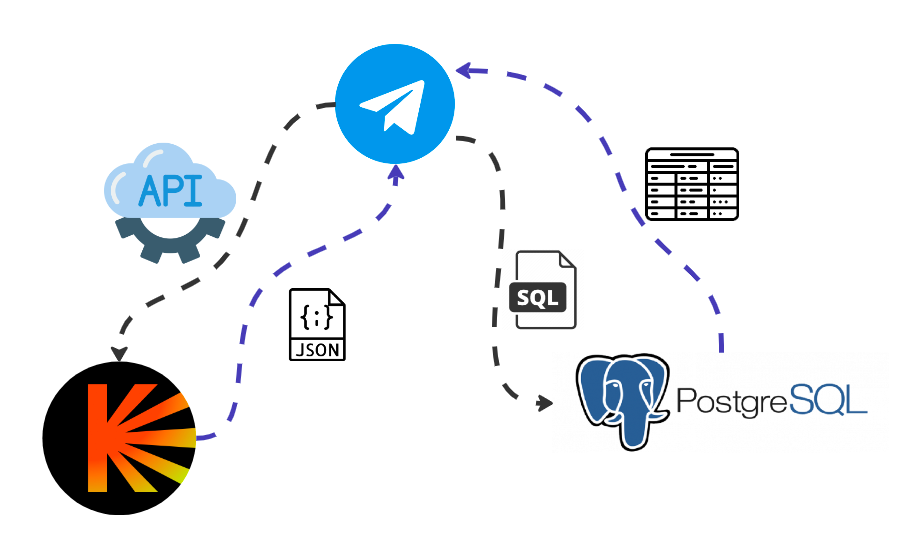
\includegraphics[width=1\textwidth]{project_structure.png}

\begin{enumerate}
    \item Бот отправляет API запрос к кинопоиску с фильтрами, чтобы тот достал фильмы/сериалы
    \item Кинопоиск возвращает ему json с результатами
    \item Бот предлагает пользователям полученные фильмы
    \item Для каждого игрока бот запоминает понравившиеся фильмы и кладет их в базу данных
    \item По запросу пользователя бот достает понравившиеся фильмы игрока
\end{enumerate}

\section{Этапы выполнения}
\begin{itemize}
    \item Написание бота, который умеет обаботать 'фильтры' игроков
    \item Добавление api запросов к пользователю без задействования базы данных
    \item Внедрение базы данных с хранением id пользователя, жанра, названия фильма и года выпуска
\end{itemize}

\section{Дальнейшее разватие}
Для развития проекта так же можно добавить функцию с запоминанием фильма/сериала независимо от того, был он в подборке фильмов во время игры или нет, а просто по желанию пользователя, в так называемый wishlist. Так же функцию удаления фильма по просьбе пользователя, если тот его уже посмотрел.

\end{document}
